Lorem ipsum dolor sit amet, quidam omnesque ea vis. Eum an aliquip legendos recusabo. Mea ex purto natum, ne movet fuisset sit. Labore audiam eos ad, facer ornatus posidonium ne ius, et eos duis delenit nusquam.

\subsection{Project Charter}
Lorem ipsum dolor sit amet, quidam omnesque ea vis. Eum an aliquip legendos recusabo. Mea ex purto natum, ne movet fuisset sit. Labore audiam eos ad, facer ornatus posidonium ne ius, et eos duis delenit nusquam.

\subsection{Product Backlog}
Lorem ipsum dolor sit amet, quidam omnesque ea vis. Eum an aliquip legendos recusabo. Mea ex purto natum, ne movet fuisset sit. Labore audiam eos ad, facer ornatus posidonium ne ius, et eos duis delenit nusquam.

\subsection{Sprint Planning}
Lorem ipsum dolor sit amet, quidam omnesque ea vis. Eum an aliquip legendos recusabo. Mea ex purto natum, ne movet fuisset sit. Labore audiam eos ad, facer ornatus posidonium ne ius, et eos duis delenit nusquam.

\subsubsection{Sprint Goal}
The main goals of this sprint are to complete project charter, meet with guy from RCT for further requirements of the product and make list of hardware parts that need to be ordered.


\subsubsection{Sprint Planning}
The sprint backlog for this sprint cycle are meeting with RCT guy for further product requirements, research about the hardware require to build the product and to complete the project charter

\subsubsection{Task Breakdown}
Lorem ipsum dolor sit amet, quidam omnesque ea vis. Eum an aliquip legendos recusabo. Mea ex purto natum, ne movet fuisset sit. Labore audiam eos ad, facer ornatus posidonium ne ius, et eos duis delenit nusquam.

\subsection{Sprint Burndown Charts}
Lorem ipsum dolor sit amet, quidam omnesque ea vis. Eum an aliquip legendos recusabo. Mea ex purto natum, ne movet fuisset sit. Labore audiam eos ad, facer ornatus posidonium ne ius, et eos duis delenit nusquam.

\begin{figure}[h!]
    \centering
    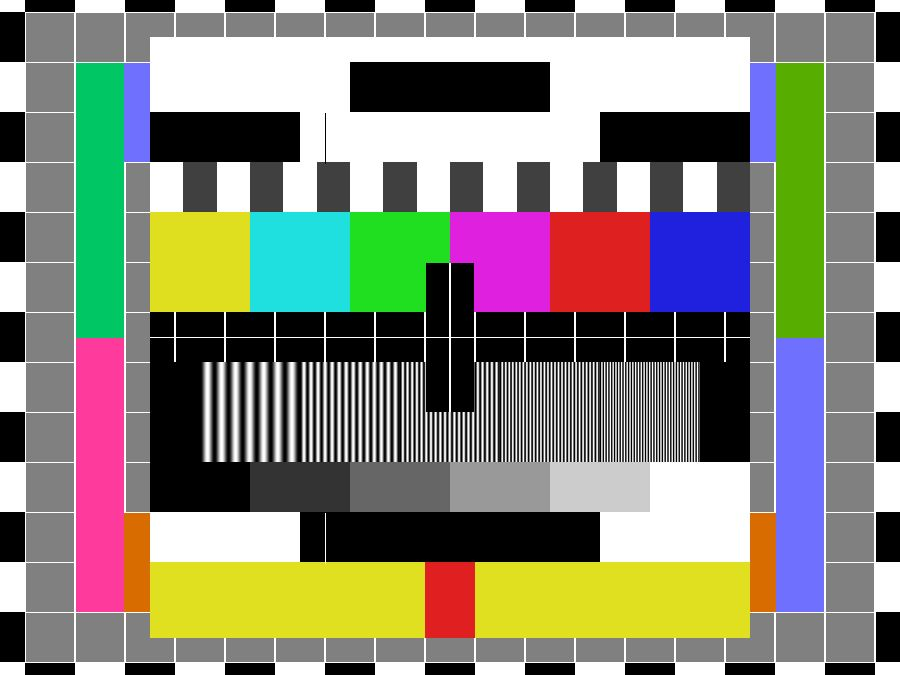
\includegraphics[width=0.5\textwidth]{images/test_image}
    \caption{Example sprint burndown chart}
\end{figure}

\subsection{Sprint Retrospective}
Lorem ipsum dolor sit amet, quidam omnesque ea vis. Eum an aliquip legendos recusabo. Mea ex purto natum, ne movet fuisset sit. Labore audiam eos ad, facer ornatus posidonium ne ius, et eos duis delenit nusquam.

\subsection{Individual Status Reports}
Lorem ipsum dolor sit amet, quidam omnesque ea vis. Eum an aliquip legendos recusabo. Mea ex purto natum, ne movet fuisset sit. Labore audiam eos ad, facer ornatus posidonium ne ius, et eos duis delenit nusquam.

\subsection{Engineering Notebooks}
Engineering notebooks will be used by all team members to record ideas, observations, designs, progress, and what was discussed in team meetings. In addition, the engineering notebook represents official documentation that could be used for patent activities or legal issues. 

\subsection{Closeout Materials}
Lorem ipsum dolor sit amet, quidam omnesque ea vis. Eum an aliquip legendos recusabo. Mea ex purto natum, ne movet fuisset sit. Labore audiam eos ad, facer ornatus posidonium ne ius, et eos duis delenit nusquam.

\subsubsection{System Prototype}
The system prototype will consist of a raspberry pi and raspberry pi camera board organized in an enclosure. 

\subsubsection{Project Poster}
The project poster will contain information regarding the project’s vision, mission, background, and the finished product’s hardware and software details. The poster will be presented at the conclusion of Computer System Design Project II in August, 2016. 

\subsubsection{Web Page}
Is this necessary?

\subsubsection{Demo Video}
A demo video will be provided to show how to appropriately use and manage the camera and the software. It will demonstrate...

\subsubsection{Source Code}
The source code will consist of software of the user interface to utilize and control the camera. In addition, the source code to allow the user to view the stream of the camera will be provided.  How will this be presented?

\subsubsection{Source Code Documentation}
The provided source code will be documented properly by including comprehensive comments to allow TrafficNet LLC or their customers to maintain and evolve the software efficiently. 

\subsubsection{Hardware Schematics}
The design files for the circuit will be provided to display what was customized in order to attain the appropriate board for the camera. How will this be presented?

\subsubsection{CAD files}
Is this necessary?

\subsubsection{Installation Scripts}
Is this necessary?

\subsubsection{User Manual}
A user manual will be provided to describe how to properly operate the camera and utilize the software. It will explain in detail the purpose of each feature of the camera and how to appropriately use them. In addition, the manual will describe the software interface and how to make changes according to the user’s preferences. How will this be presented? 


